% BFS depth wall, one curve per tier.
% Cost model: t(d) = b^d * c0 * g^d, with the per-node enumeration cost measured
% Generated by workspace/figures/make_depth_wall_figure.mjs
% Source: workspace/depth_wall/depth_wall.csv
% easy: b = 2.721, g = 1.441, c0 = 4.26e-3s (b*g = 3.92, 14 profiled states), reference depth 6.8, predicted 46 s (b fitted on 7 budget-exhausted runs over 3 samples)
% mid: b = 3.147, g = 1.472, c0 = 1.49e-2s (b*g = 4.63, 11 profiled states), reference depth 12.0, predicted 17 d (b fitted on 12 budget-exhausted runs over 3 samples)
% hard: b = 7.050, g = 1.758, c0 = 3.18e-1s (b*g = 12.39, 12 profiled states), reference depth 19.0, predicted 5.9e+12 y (b fitted on 8 budget-exhausted runs over 2 samples)
%
% Standalone: pdflatex depth_wall.tex
% In a paper: keep the tikzpicture, drop the documentclass wrapper.
\documentclass[border=2pt]{standalone}
\usepackage{pgfplots}
\pgfplotsset{compat=1.18}
\begin{document}
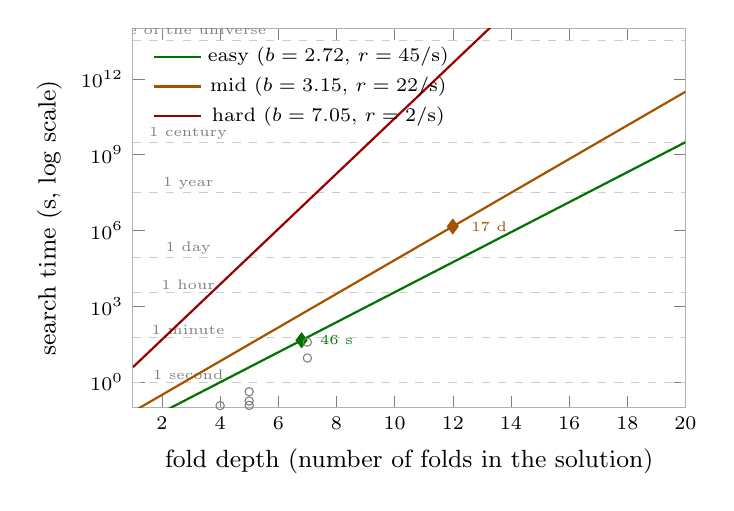
\begin{tikzpicture}
\begin{axis}[
  width=8.6cm, height=6.4cm,
  ymode=log,
  xlabel={fold depth (number of folds in the solution)},
  ylabel={search time (s, log scale)},
  xmin=1, xmax=20, ymin=1e-1, ymax=1e14,
  xtick={2,4,6,8,10,12,14,16,18,20},
  ytick={1e0,1e3,1e6,1e9,1e12},
  tick label style={font=\scriptsize},
  label style={font=\small},
  legend style={font=\scriptsize, at={(0.02,0.98)}, anchor=north west, draw=none, fill=none},
  axis line style={gray!60},
]
\draw[gray!40, dashed, thin] (axis cs:1,1.0000e+0) -- (axis cs:20,1.0000e+0)
  node[pos=0.10, above, font=\tiny, gray, inner sep=1pt] {1 second};
\draw[gray!40, dashed, thin] (axis cs:1,6.0000e+1) -- (axis cs:20,6.0000e+1)
  node[pos=0.10, above, font=\tiny, gray, inner sep=1pt] {1 minute};
\draw[gray!40, dashed, thin] (axis cs:1,3.6000e+3) -- (axis cs:20,3.6000e+3)
  node[pos=0.10, above, font=\tiny, gray, inner sep=1pt] {1 hour};
\draw[gray!40, dashed, thin] (axis cs:1,8.6400e+4) -- (axis cs:20,8.6400e+4)
  node[pos=0.10, above, font=\tiny, gray, inner sep=1pt] {1 day};
\draw[gray!40, dashed, thin] (axis cs:1,3.1558e+7) -- (axis cs:20,3.1558e+7)
  node[pos=0.10, above, font=\tiny, gray, inner sep=1pt] {1 year};
\draw[gray!40, dashed, thin] (axis cs:1,3.1558e+9) -- (axis cs:20,3.1558e+9)
  node[pos=0.10, above, font=\tiny, gray, inner sep=1pt] {1 century};
\draw[gray!40, dashed, thin] (axis cs:1,3.1558e+13) -- (axis cs:20,3.1558e+13)
  node[pos=0.10, above, font=\tiny, gray, inner sep=1pt] {age of the universe};
\addplot[thick, color=green!45!black, mark=none] coordinates {
  (1,1.66830e-2)
  (2,6.54005e-2)
  (3,2.56383e-1)
  (4,1.00507e+0)
  (5,3.94007e+0)
  (6,1.54458e+1)
  (7,6.05506e+1)
  (8,2.37370e+2)
  (9,9.30537e+2)
  (10,3.64789e+3)
  (11,1.43004e+4)
  (12,5.60604e+4)
  (13,2.19768e+5)
  (14,8.61532e+5)
  (15,3.37737e+6)
  (16,1.32399e+7)
  (17,5.19032e+7)
  (18,2.03470e+8)
  (19,7.97644e+8)
  (20,3.12692e+9)
};
\addlegendentry{easy ($b=2.72$, $r=45$/s)}
\addplot[thick, color=orange!65!black, mark=none] coordinates {
  (1,6.89243e-2)
  (2,3.19313e-1)
  (3,1.47932e+0)
  (4,6.85338e+0)
  (5,3.17504e+1)
  (6,1.47093e+2)
  (7,6.81456e+2)
  (8,3.15705e+3)
  (9,1.46260e+4)
  (10,6.77595e+4)
  (11,3.13917e+5)
  (12,1.45432e+6)
  (13,6.73756e+6)
  (14,3.12138e+7)
  (15,1.44608e+8)
  (16,6.69939e+8)
  (17,3.10370e+9)
  (18,1.43788e+10)
  (19,6.66144e+10)
  (20,3.08611e+11)
};
\addlegendentry{mid ($b=3.15$, $r=22$/s)}
\addplot[thick, color=red!60!black, mark=none] coordinates {
  (1,3.94464e+0)
  (2,4.88768e+1)
  (3,6.05619e+2)
  (4,7.50405e+3)
  (5,9.29805e+4)
  (6,1.15209e+6)
  (7,1.42753e+7)
  (8,1.76881e+8)
  (9,2.19168e+9)
  (10,2.71564e+10)
  (11,3.36487e+11)
  (12,4.16932e+12)
  (13,5.16608e+13)
  (13.5,1.81848e+14)
};
\addlegendentry{hard ($b=7.05$, $r=2$/s)}
\addplot[only marks, mark=diamond*, mark size=2.6pt, color=green!45!black, forget plot]
  coordinates {(6.80,4.60741e+1)};
\node[font=\tiny, color=green!45!black, anchor=west] at (axis cs:7.10,4.60741e+1) {46 s};
\addplot[only marks, mark=diamond*, mark size=2.6pt, color=orange!65!black, forget plot]
  coordinates {(12.00,1.45432e+6)};
\node[font=\tiny, color=orange!65!black, anchor=west] at (axis cs:12.30,1.45432e+6) {17 d};
\addplot[only marks, mark=diamond*, mark size=2.6pt, color=red!60!black, forget plot]
  coordinates {(19.00,1.86955e+20)};
\node[font=\tiny, color=red!60!black, anchor=west] at (axis cs:19.30,1.86955e+20) {5.9e+12 y};
\addplot[only marks, mark=o, mark size=1.5pt, color=gray, forget plot] coordinates {
  (4,1.20000e-1)
  (5,4.25000e-1)
  (5,1.82000e-1)
  (5,1.23000e-1)
  (7,9.14900e+0)
  (7,3.87370e+1)
};
\end{axis}
\end{tikzpicture}
\end{document}
